%\documentclass[]{spie}  %>>> use for US letter paper
\documentclass[a4paper,nocompress]{spie}  %>>> use this instead for A4 paper
%\documentclass[nocompress]{spie}  %>>> to avoid compression of citations

\renewcommand{\baselinestretch}{1.0} % Change to 1.65 for double spacing
 
\usepackage{amsmath,amsfonts,amssymb}
\usepackage{graphicx}
\usepackage[colorlinks=true, allcolors=blue]{hyperref}
\usepackage[dvipsnames]{xcolor}
\usepackage{tabularx}
\usepackage{wrapfig}
\setlength{\extrarowheight}{2pt}
\usepackage{chemformula}

\title{Quantifying the Impact \\ of Performance Improvements and Cost Reductions \\ from 20 years of Light-Emitting Diode Manufacturing}

\author[a,b]{Michael Weinold}
\author[a]{Sergey Kolesnikov}
\author[a,c]{Laura Diaz Anadon}
\affil[a]{Centre for Environment, Energy and Natural Resource Governance, Department of Land Economy, University of Cambridge, Cambridge, CB3 9EP, UK}
\affil[b]{Chair of Entrepreneurial Risks, ETH Zurich, Scheuchzerstrasse 7, CH-8092 Zurich, CH}
\affil[c]{Belfer Center for Science and International Affairs, Harvard Kennedy School, Harvard University, Cambridge, MA 02138, USA}

\authorinfo{Further author information: (Send correspondence to Michael Weinold) \\ MW: E-mail: mw799@cam.ac.uk \\ SK: E-mail: sk2063@cam.ac.uk \\ LDA: E-mail: lda24@cam.ac.uk}

% Option to view page numbers
\pagestyle{empty} % change to \pagestyle{plain} for page numbers   
\setcounter{page}{301} % Set start page numbering at e.g. 301
 
\begin{document} 
\maketitle

\begin{abstract}
    
    With the aim of identifying and quantifying the principal sources of performance improvements and cost reductions in white light emitting diode manufacturing, we collect historical data on device cost and performance, technological breakthroughs and manufacturing innovation for phosphor-converted white light-emitting diodes for the past 20 years. We find that technological breakthroughs and process innovation contributed to performance improvements across the entire range of LED device sub-efficiencies, resulting in the overall increase in the lamp efficiency for the highest performing devices at a test current of 350mA from 5.8\% to 38.7\% between 2002 and 2020. We further develop a bottom-up manufacturing cost model with process-step resolution that captures improvements in throughput, yield and related costs of all relevant manufacturing steps, as well as economies of scale, to analyse progress in LED manufacturing cost structure between early manufacturing in 2002 and mature industry in 2020. We estimate that the cost of manufacturing low-power and mid-power light-emitting diode packages at a US location using state-of-the-art equipment has dropped from 1.11\$(2020) in 2002 to 0.05\$(2020) in 2020, a 95.5\% decrease. We also find that the largest contribution to overall cost reduction has come from increase in wafer size, and that in 2020, LED chip packaging is the largest contributor to cost at 60\%.

\end{abstract}

% Include a list of keywords after the abstract 
\keywords{light-emitting diodes, LED manufacturing, LED efficiency, manufacturing cost, cost modeling, cost reduction, technological breakthroughs}

\section{INTRODUCTION}
\label{sec:intro}


    Within just 25 years of the introduction of first commercial white light-emitting diodes (LED), the solid state lighting (SSL) industry has become a rare success story in the global drive for the transformation of energy systems. Today, the solid-state lighting markets in the US and the EU together are valued at 58.7 Bn.\$(2020) \cite{gvr2020market_us,gvr2020market_eu} with general illumination market penetration exceeding 50\% \cite{eu2019impactass,stratunl2018}. Estimates for the electrical energy saved annually from SSL adoption range from 131 TWh/year in 2020 for the EU \cite{eu2019impactass} to 442 TWh/year in 2020 for the US \cite{yamada2015adoption,guidehouse2020adoption}, which is on par with the amount of energy produced by all deployed solar photovoltaic installations in these regions. This revolution in lighting would not have been possible without dramatic improvements in the overall LED device efficiency and reductions in LED manufacturing costs.

    Understanding the sources and impact of these improvements on LED manufacturing is essential for researchers, industry professionals, as well as policymakers in the sphere of energy, science and innovation, as they may provide valuable insights for the acceleration of innovation in other demand-side energy technologies. With this aim, in this paper we identify and quantify the principal sources of performance improvements and cost reductions in phosphor-converted white LED lighting devices over the last 20 years. 

\section{Methods and Data}
\label{sec:methods}

\subsection{Choice of Metrics}
\label{subsec:metrics}

    To quantify the effect of technological breakthroughs and manufacturing process improvements, a set of metrics has to be identified that describes all dimensions of device performance, including the overall physical device efficiency and the sub-efficiencies related to different physical loss channels. They must further have the ability to directly capture the effect of individual technological breakthroughs, evolution in device architecture, and manufacturing process improvements on device performance.
    
    These requirements precluded the use of some established metrics. For instance, a highly cited and frequently updated metric is the total luminous flux per light-emitting diode package \cite{Liu2009,haitz2011solid,cho2017white,Fontoynont2018}. In combination with the cost per total flux, it is sometimes referred to as \textit{"Haitz's Law"}, in reference to an early report on LED development by Haitz et al. \cite{haitz1999case}. However, while it is often used to showcase technological progress in light-emitting diode design and manufacturing, care must be taken to consider its limitations.
    
    \begin{figure} [ht]
        \begin{center}
            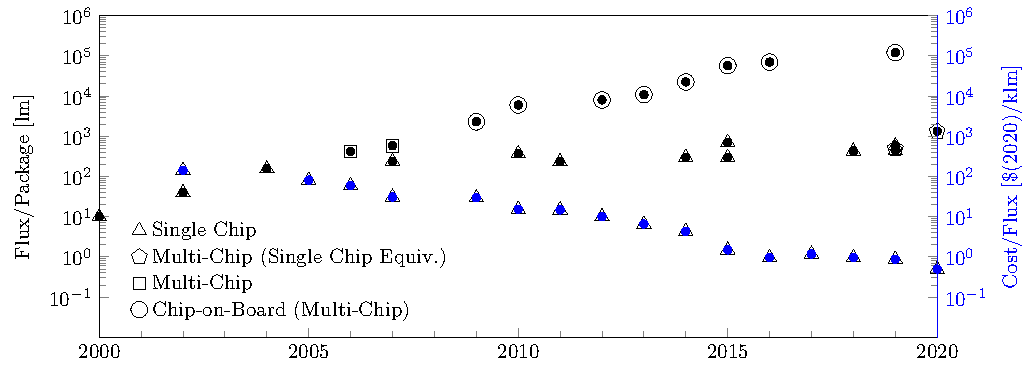
\includegraphics[width=\textwidth]{haitz_law_white.pdf}
        \end{center}
        \caption{Historical increase in flux for the highest-performing white light-emitting diode chips and (multi-chip) packages, inspired by \textit{"Haitz's Law"}\cite{haitz1999case}. Shown are the datapoints for best commercial performers gathered from press releases, datasheets and industry periodicals. Note the logarithmic ordinates, black-colored datapoints corresponding to the left ordinate, and blue-colored datapoints corresponding to the right ordinate.}
        \label{fig:haitz}
    \end{figure}
    
    Firstly, today, the metric retains only limited significance as an appropriate proxy for technological progress in light-emitting diodes. This is because it is not desirable to increase the total flux per device beyond a certain point in many applications. Reasons for limiting the total flux per device may include lighting design considerations to reduce glare \cite{khan2015led}, device efficiency considerations to avoid electrical droop at high operating currents associated with high brightness \cite{Piprek2010}, and economical considerations that multiple LED chips in a single package can achieve the same brightness as a single high-brightness LED die. Secondly, the total flux per device would only be a proxy for technological improvements in light-emitting diodes if data was given for single light-emitting diode chips instead of multi-chip packages. Historically, publications have sometimes failed to make this distinction, listing datapoints for both device levels in the same graph without supporting information.

    Figure \ref{fig:haitz} shows an updated and expanded overview of the flux per device and the cost per flux of highest performing light-emitting diodes, both at the chip and package level, to demonstrate the limitations of these metrics. It is evident that the historical improvements in total flux per package for single chips are not as pronounced as for multi-chip packages.

    Instead, progress in light-emitting diode technology is best described by the overall device efficiency, or lamp efficiency. This metric is defined as the product of all device sub-efficiencies associated with an ensemble of different loss channels $\eta_L = \prod_{i=(V_f,\dots,S)} \eta_i$. Sub-efficiencies directly capture the effect of particular technological breakthroughs in device design and manufacturing process improvements. Table \ref{tab:eff} lists the relevant sub-efficiencies considered in our work, along with their mathematical definitions.
    
        \begin{table}[h!]
        \caption{List of LED device sub-efficiencies used in our methodology. We follow the definitions used by Tsao et al. \cite{tsao2010solid} and Pattison et al. \cite{pattison2017solid}. Historical developments in the sub-efficiencies are displayed in figure \ref{fig:efficiency}.}
        \bigskip
        \centering
    	\begin{tabularx}{\textwidth}{|l|l|l|X|}
    		\hline
    			\textit{Symbol} & \textit{Sub-Efficiency} & \textit{Loss-Channel} & \textit{Definition} \\
    		\hline
    		    $\eta_{V_f}$ & Forward Voltage Efficiency* & Ohmic Resistance & $\eta_{V_f} = E_{h\nu} / V_f $ \\
    		\hline
    		    $\eta_{LE}$ & Light-Extraction Efficiency & Re-absorption and Reflection & $\eta_{LE}= P_{out} / P_{in} $ \\
    		\hline
    		    $\eta_{IQ}$ & Internal Quantum Efficiency & Non-radiative Recombinations & $\eta_{EQ} = \eta_{IQ} \times \eta_{LE}$ \\
    		\hline
    		    $\eta_{Droop}$ & (Electrical) Droop & Non-radiative Recombinations & $\eta_{Droop} = 1 - \eta_{IQE} / \eta_{IQE}(A \rightarrow 0) $ \\
    		\hline
    		    $\eta_C$ & Conversion Efficiency & Stokes Loss, Absorption, etc. & $\eta_{C} = E_{\textcolor{blue}{B}} / \sum_{i=\textcolor{red}{R},\textcolor{orange}{O},\textcolor{yellow}{Y},\textcolor{teal}{G}} E_i$ \\
    		\hline
    		    $\eta_{S}$ & Spectral Efficiency & Eye Sensitivity & $\eta_{S} = K / K_{max}(CRI,CCT)$ \\
    		\hline
    		    $\eta_L$ & Lamp Efficiency & N/A (Cumulative) & $\eta_L = \prod_{i=(V_f,\dots,S)} \eta_i$ \\
            \hline
                \multicolumn{4}{|l|}{$\!\begin{aligned}
                    E_{h\nu} &\dots \text{photon energy} \\
                    V_f &\dots \text{forward voltage} \\
                    A &\dots \text{electrical current} \\
                    E_{B,\dots,G} &\dots \text{optical energy of monochromatic light (blue, red, orange, yellow, green)} \\
                    K &\dots \text{luminous efficacy of radiation} \\
                    CRI &\dots \text{color rendering index}, \ CCT \dots \text{color temperature} \\
                \end{aligned}$} \\
            \hline
    	\end{tabularx}
    	\label{tab:eff}
    \end{table}
    
    Performance improvements in metrics related to consumer experience have also played a role in the adoption of LED-based luminaires \cite{cowan2011understanding}. Broadly described as the quality of light, these include metrics related to the emitted spectrum, as well as flicker, the temporal modulation of light. For instance, breakthroughs in the development of down-conversion phosphors enabled a greater range in the color temperature of light sources. The analysis of consumer experience metrics is ongoing and will be presented in our future research. Notably, we exclude flicker from this work because it is an inherent property not of the light-emitting diodes themselves, but rather the electrical ballasts in the luminaires. For further discussion of flicker in this context, see a recent publication by Weinold \cite{weinold2020long}.

    \subsection{Data Sources and Performance Calculations}
    \label{subsec:data}
    
        To gain a detailed understanding of the sources and magnitude of efficiency improvements and cost reductions in LED manufacturing, we gathered historical data on device cost and performance across different sub-efficiencies, as well as on technological breakthroughs and manufacturing innovation for phosphor-converted white light-emitting diodes for the past 20 years. The data was collected from a variety of sources such as patent literature, scientific articles, company publications, industry reports and roadmaps, and technical periodicals. Additional information was provided by experts from academia, the LED manufacturing industry, and the manufacturing equipment industry during semi-structured interviews. We further had to identify the associated device architectures, manufacturing processes and types of down-conversion phosphors used. 
        
        \begin{figure} [ht]
            \begin{center}
                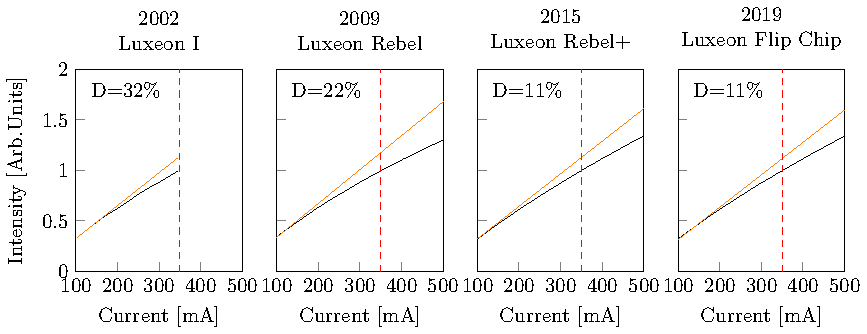
\includegraphics[width=0.85\textwidth]{SPIE/article/droop_lumileds.pdf}
            \end{center}
            \caption{Luminous intensity of four different \textit{Lumileds} high-power light-emitting diodes normalized to the value at a test current of $A_{test}=350$mA. The black curves describe the real measured intensity, the orange curves describe the estimated ideal intensity. Droop $D$, as defined in table \ref{tab:eff}, is the difference between these curves at the test current. Current-Intensity data extracted from device datasheets \cite{datasheet_lumileds_lux1,datasheet_lumileds_rebel,datasheet_lumileds_rebplus,lumi2019data}}
            \label{fig:droop}
        \end{figure}
        
        In cases where efficiency data was not readily available, we calculated the respective values from raw performance data. For instance, to calculate historical data on the reduction of losses associated with electrical droop, we used device performance data extracted from datasheets by the method shown in figure \ref{fig:droop}. This data was cross-referenced with information on the different chip architectures and manufacturing processes used for each device. In a similar way, data was gathered for all sub-efficiencies listed in table \ref{tab:eff} to gain a complete picture of the historical developments in light-emitting diode efficiency.

    \subsection{Manufacturing Cost Model}
    \label{subsec:costmodel}
    

        To quantify changes in the manufacturing cost of LED devices, a bottom-up manufacturing cost model with process step resolution was constructed. It covers the entire manufacturing process of GaN-on-sapphire-based phosphor-converted low-to-mid power light-emitting diode packages of different chip architectures. We designed it to accommodate the classical p-side-up lateral current spreading architecture, with two further architectures\textemdash a packaged flip-chip vertical current spreading architecture and a chip-scale package flip chip architecture\textemdash under development. An excerpt of the evolution of the classical chip architecture considered in the cost model is shown in figure \ref{fig:chip_arch}. The earliest commercial warm-white phosphor converted blue light emitting diodes were introduced in 2002, so the model was constructed for the years 2002, 2012 and 2020. It was populated with equipment data from European and North American firms, selected for a virtual North American manufacturing location. Details of the manufacturing processes and process-specific step parameters were derived from the sources mentioned in section \ref{subsec:data}. For 2012, additional data for the model was adapted from the \textit{LEDCOM} cost model prepared for the US Department of Energy by Stephen Bland of SB Consulting\cite{ledcomv2}. Our model includes the wafer treatment process with further ongoing work also focusing on the chip packaging process. While the model offers great flexibility in adapting the manufacturing process parameters and chip architectures used, it is important to note the limitations of this approach. The main aim of the model is not to faithfully represent real-world manufacturing such as in present-day manufacturing locations in Asia, but rather to show the effect of technological change and manufacturing process improvements on total cost. 

        \begin{figure} [ht]
            \begin{center}
                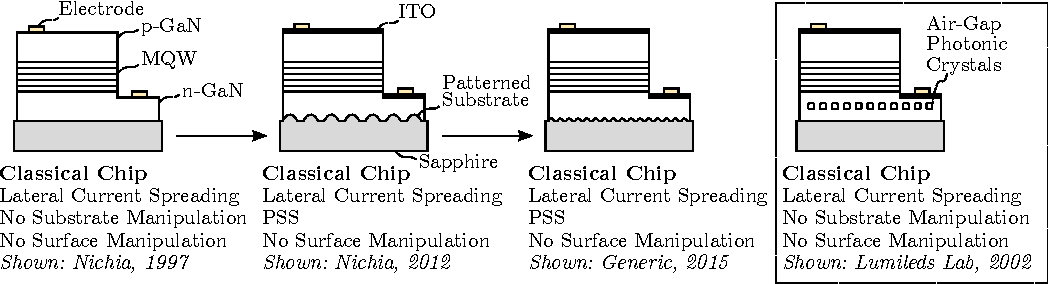
\includegraphics[width=\textwidth]{SPIE/article/chip_architectures.pdf}
            \end{center}
            \caption{Cutaway side views of the evolution of chip architectures for classical chip designs (lateral current spreading). Note that dimensions are not to scale. Years correspond to earliest identified patent priority date. Illustration in the box indicates a chip design not brought to large scale production. Drawings adapted from patents \cite{nagahama2013nitride,tanaka2010semiconductor,wierer2006photonic}}
            \label{fig:chip_arch}
        \end{figure}

        To disaggregate the contribution of changes in single variables to changes in the total manufacturing cost, we used an approach introduced by Kavlak and colleagues in a cost model for photovoltaic modules \cite{kavlak2018evaluating}. It is based on the logarithmic derivative of the total differential of the cost function. For the detailed derivation, we refer to the supplementary material of the original publication.

\section{RESULTS}

\subsection{Performance Improvements}

     Main results for performance improvements are presented in Figure \ref{fig:efficiency}. Overall efficiency in best performing devices improved from $\eta_L=5.8\%$ in 2002 to $\eta_L = 38.7\%$ in 2020. As previous studies have noted, no single loss channel dominates the overall the efficiency\cite{tsao2010solid}. Figure \ref{fig:efficiency} additionally shows the physical limits for the loss channels. We find that those loss channels with a fixed physical limit below 100\% have become significantly more dominant in 2016 and 2020. An example of this tendency is the increased importance of Stokes loss that describes the energy dissipated upon conversion from short wavelength to long wavelength photons. Notably, sub-efficiencies for the most current devices are only $\sim10\%$ below the physical limit. The exception is spectral efficiency, which at $\sim17\%$ below the physical limit shows larger potential for improvement.
     
     Our comparison between the improvements in device sub-efficiencies between 2002 and 2020 shows that the aggregate efficiency improvement was not driven primarily by improvements in a single sub-efficiency. Instead, there has been consistent progress across the ensemble of loss channels corresponding to the device sub-efficiencies in the past 18 years, including forward voltage efficiency ($70\%\rightarrow99.5\%$), internal quantum efficiency ($55\%\rightarrow90\%)$, electrical droop ($65\%\rightarrow90\%$), light-extraction efficiency ($60\%\rightarrow90\%$) and spectral efficiency ($74\% \rightarrow83\%$).
     
    \begin{figure} [ht]
        \begin{center}
            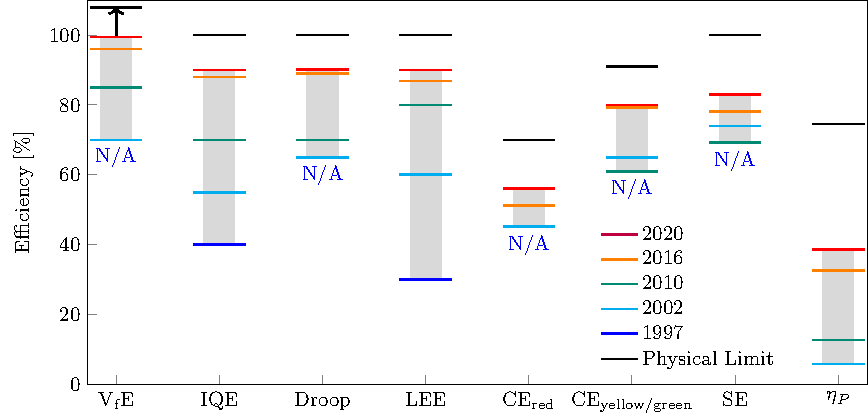
\includegraphics[width=0.85\textwidth]{SPIE/article/breakthroughs_efficiency.pdf}
        \end{center}
        \caption{Historical changes in sub-efficiencies of phosphor-converted warm white light-emitting diodes with test currents of at least $I_\text{test}=350$mA. The overall lamp efficiency $\eta_L$ is displayed as the rightmost column. This figure takes as inputs the state-of-the-art sub-efficiencies discussed in section \ref{subsec:metrics}. Horizontal colored bars give state-of-the-art sub-efficiencies for five years: \textcolor{blue}{1997}, \textcolor{teal}{2002}, \textcolor{orange}{2010}, \textcolor{magenta}{2016} and \textcolor{red}{2020}. Colored annotation "N/A" indicates that the sub-efficiency of the corresponding year cannot be computed for the following reasons: V$_\text{f}$E, Droop: depend on current, which was below 350mA at the time; CE, SE: warm white spectrum LEDs not available at the time. Physical limits are indicated by black horizontal bars. Possible range for the physical limit of V$_\text{f}$E exceeds 100\%, depends on electrical device parameters, and is indicated by an upward pointing black arrow. Efficiency acronyms are listed in table \ref{tab:eff}.}
        \label{fig:efficiency}
    \end{figure}
    
    Notably, improvements in sub-efficiencies with a good understanding of the underlying physical loss channels, such as light-extraction efficiency, forward voltage efficiency and spectral efficiency, were mostly a result of targeted research and development. For instance, optical simulations could be performed to determine ways of modifying the device architecture to improve light extraction efficiency. On the other hand, efficiency improvements in sub-efficiencies with a relatively limited understanding of underlying physical mechanisms, such as internal quantum efficiency and the associated electrical droop at high currents, were mostly due to manufacturing process improvements. For instance, the reasons for electrical droop have, until recently, been a topic of hot debate. Despite that, significant improvements in this channel were still achieved by varying metal-organic vapour deposition (MOCVD) growth parameters in large ensembles of wafer batches.

\subsection{Manufacturing Cost Reductions}
    
    Results of manufacturing cost modeling for three reference years (2002, 2012, and 2020), broken down by five main cost components in our model\textemdash substrate, epitaxy, wafer processing, chip packaging, and phosphor\textemdash are presented in table \ref{tab:cost}. Using our cost model, we estimate that the cost of manufacturing low-to-mid-power light-emitting diode packages at a US location, using state-of-the-art equipment, have declined from 1.11\$(2020) in 2002 to 0.05\$(2020) in 2020, a 95.5\% overall cost reduction. 
    
    A preliminary analysis of the cost model components suggests that an increase in the wafer size is responsible for the largest part of the overall cost reduction. The wafer diameter $d$ used in production has been steadily increasing since 2002. The model assumes diameters and associated number of die per wafer changing from $d(2002)=50$mm$\rightarrow851$ to $d(2020)=200$mm$\rightarrow26,838$. Related decreases in exclusion zone and cutting width have also contributed to the increase in die per wafer number. Further analysis of the relative contributions of different manufacturing process steps to the cost structure suggests that as the number of die per wafer increases, the packaging steps now carry the largest share of the total cost at 60\% in 2020. This is because the output of these steps is limited by the throughput of the associated equipment. The wafer processing steps, which made the largest contribution to the total cost in 2002, depend on the number of die per wafer and only to a lesser extent on the throughput of equipment, which explains why they became relatively less important in the cost structure by 2020.
    
    \begin{table}[h!]
        \caption{Manufacturing cost of low-power classical chips (lateral current spreading) estimated with the cost model introduced in section \ref{subsec:costmodel}.}
        \bigskip
            \centering
            \begin{tabularx}{\textwidth}{|l|l|X|X|X|X|X|l|}
            	\hline
            		\textit{Year} & \textit{Unit} & \textit{Substrate} & \textit{Epitaxy} & \textit{Wafer Proc.} & \textit{Packaging} & \textit{Phosphor} & \textit{Total} \\
                \hline
                    2002 & \$(2020) & 0.0760 & 0.1638 & 0.7351 & 0.1203 & 0.0175 & 1.1131 \\
                \hline
                    2002-2012 & $\Delta$ \% & -98.8 & -94.7 & -96.2 & -47.8 & -42.2 & -90.1 \\
                \hline
                    2012 & \$(2020) & 0.0008 & 0.0086 & 0.0276 & 0.0627 & 0.0101 & 0.0111 \\
                \hline
                    2012-2020 & $\Delta$ \% & -81.8 & -34.37 & -61.5 & -50.3 & -56.4 & -52.7 \\
                \hline
                    2020 & \$(2020) & 0.0001 & 0.0056 & 0.0106 & 0.0311 & 0.0044 & 0.0528 \\
                \hline
            \end{tabularx}
            \label{tab:cost}
        \end{table}


\section{CONCLUSIONS}

    In this study, we found that technological breakthroughs and manufacturing process innovation contributed to performance improvements across the entire range of LED device sub-efficiencies, resulting in the overall lamp efficiency increase for the highest performing devices at a test current of 350mA from 5.8\% in 2002 to 38.7\% in 2020. Notably, we found that efficiency improvements in loss channels with a good understanding of underlying physical mechanisms were driven mostly by research and development, while improvements in channels with a lack of such understanding required extensive experimentation and learning-by-doing in the manufacturing setting. It shows the importance of further research into the underlying solid-state physics of light-emitting diodes. A deeper understanding of the effects and mechanisms associated with device loss channels will potentially enable further advances in LED technology, with spectral efficiency in particular showing promise for further improvements. 

    We also constructed the manufacturing cost model for low-to-mid-power LED packages produced at a virtual US location using state-of-the-art equipment. We estimated that the cost of LED manufacturing in these conditions decreased by 95.5\% from 1.11\$(2020) in 2002 to 0.05\$(2020) in 2020. The largest contribution to the overall cost reductions came from increase in the wafer size, while the largest remaining contributor to the manufacturing cost is the LED packaging, which accounts for 60\% of the cost structure in 2020.

\acknowledgments % equivalent to \section*{ACKNOWLEDGMENTS}       

We would like to thank Gabriel Chan, Anna Goldstein and Venkatesh Narayanamurti for many helpful discussions and their feedback. We also express our deep gratitude to all interviewees for their willingness to participate in this study and invaluable contributions. This research is funded by the \textit{Alfred P. Sloan Foundation}, grant number 253128. Michael Weinold further gratefully acknowledges support from the \textit{Swiss Study Foundation} of Zurich, Switzerland.

\clearpage
% References
\bibliography{report} % bibliography data in report.bib
\bibliographystyle{spiebib} % makes bibtex use spiebib.bst

\end{document} 
